%%%%%%%%%%%%%%%%%%%%%%%%%%%%%%%
\chapter{IncNavierStokesSolver: Solving the Incompressible Navier-Stokes Equations}

In this chapter, we walk the reader through our 2D and 3D incompressible Navier-Stokes Solver (IncNavierStokesSolver).

\section{Immersed Boundary Methods: Smoothed Profile Method}

The usual way to solve any PDE requires the definition of a well defined domain where the solution is to be determined. Thus, for complex geometries, the meshing process may get cumbersome and, in any case, the solver will have to cope with deformed and skewed cells, at least to some point. In addition, when solving cases with moving boundaries, the mesh has to be updated every time step to follow the the shape of the boundaries, leading to a very resource and time-consuming simulation that limits the capabilities of the solver.

Immersed Boundary Methods may turn very useful in these situations, where the definition of the boundaries requires a very complex mesh to achieve convergence. The main idea behind them is the use of a forcing term in the incompressible Navier-Stokes equations in such a way that the mesh does not necessariliy follow the boundaries. The solution in the regions falling outside the boundaries is simply that of the boundaries, forcing the the flow to behave as if there were a real object even if the mesh does not represent it. As shown in \cite{LuoSPM}, the boundaries defined in this way are no-slip walls and, in any case, the flow is still incompressible. Starting from the usual equations, the term $\BM{f_s}$ is added in the right hand side:

\begin{subequations}
\begin{equation} \label{spm:eq:SPMeqmov}
    \partf{\BM{u}}{t} + \BM{u}\cdot\nabla\BM{u} = -\nabla p + \nu\nabla^2\BM{u} + \BM{f} + \BM{f_s}
\end{equation}
\begin{equation}
    \nabla\cdot\BM{u} = 0
\end{equation}
\end{subequations}

The definition of this term depends on the method but, for the Smoothed Profile Method (SPM), is related to a \emph{shape function} $\Phi(\BM{x}, t)$ valued 0 in the fluid domain and 1 outside. It is usually defined as:

\begin{equation} \label{spm:eq:mask}
    \Phi(\BM{x}, t) = -\frac{1}{2}\left[\tanh\left(\frac{d(\BM{x}, t)}{\xi}\right)-1\right],
\end{equation}

\begin{figure}[htb]
    \centering
    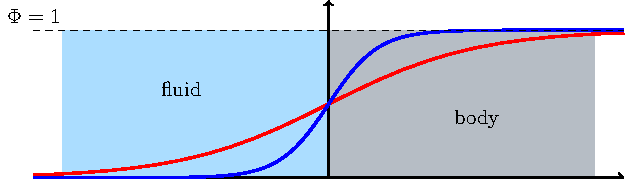
\includegraphics[width=10cm]{img/concentration.pdf}
    \caption{Definition of the shape function $\Phi$ close to the boundary of an immersed body.}
    \label{spm:fig:shapefunc}
\end{figure}

being $\xi$ a scaling factor \cite{WangSPM} and $d(\BM{x}, t)$ a function representing the distance to the boundary (positive inside the body, negative inside the fluid). If the case to be simulated includes more than one immersed boundaries, the final shape function is calculated by adding the individual ones as long as they do not overlap:

\begin{equation}
    \Phi = \sum_i \Phi_i
\end{equation}

The approach followed during the implementation in \nek is an extension of the Velocity Correction Scheme, using the final velocity obtained with this method as an intermediate velocity to determine the value of the forcing term. The initial equation \eqref{spm:eq:SPMeqmov} is slightly modified and integrated in time by means of a \emph{stiffly-stable} scheme and, then, splitted into different smaller parts that are solved separately:

\begin{equation}
     \frac{\gamma_0\BM{u}^{n+1}-\sum_{q=0}^{J-1}\alpha_q~\BM{u}^{n-q}}{\Delta t} = -\sum_{q=0}^{J-1}\beta_q~(\BM{u}\cdot\nabla\BM{u})^{n-q} -\nabla (p^*+p_p)^{n+1} + \nu\nabla^2\BM{u}^{n+1} + \BM{f}^{n+1} + \BM{f_s}^{n+1}
\end{equation}

\begin{subequations}
\begin{gather}
    \frac{\BM{\tilde{u}}-\sum_{q=0}^{J-1}\alpha_q~\BM{u}^{n-q}}{\Delta t} = -\sum_{q=0}^{J-1}\beta_q~(\BM{u}\cdot\nabla\BM{u})^{n-q} + \BM{f}^{n+1},\\
    \frac{\BM{\hat{u}}-\BM{\tilde{u}}}{\Delta t} = -\nabla {p^*}^{n+1},\\[3mm]
    \frac{\gamma_0\BM{u^*}-\BM{\hat{u}}}{\Delta t} = \nu\nabla^2\BM{u}^{n+1},\\[3mm]
    \frac{\gamma_0\BM{u}^{n+1}-\gamma_0\BM{u^*}}{\Delta t} = -\nabla p_p^{n+1} + \BM{f_s}^{n+1}
\end{gather}
\end{subequations}

The new term $\BM{f_s}$ is defined as follows:

\begin{equation}
    \BM{f_s}^{n+1} = \frac{\gamma_0\Phi^{n+1}(\BM{u_p}^{n+1}-\BM{u^*})}{\Delta t},
\end{equation}

where $\alpha_q$, $\beta_q$ and $\gamma_0$ are coefficients of the stiffly-stable time integration method and $\BM{u_p}$ is the velocity of the points that lay outside the boundaries. Thus, the new term is just an acceleration proportional to the difference between the expected and the intermediate velocity, forcing the flow to follow the shapes defined by $\Phi$ and $\BM{u_p}$. Some transformations in these expressions lead to the final SPM equations:

\begin{enumerate}
    \item Advection and external forces:
        \begin{equation}
            \frac{\BM{\tilde{u}}-\sum_{q=0}^{J-1}\alpha_q~\BM{u}^{n-q}}{\Delta t} = \sum_{q=0}^{J-1}\beta_q\left[-\BM{u}\cdot\nabla\BM{u}+\BM{f}\right]^{n-q}
        \end{equation}
    \item Pressure:
        \begin{subequations}
        \begin{gather}
            \nabla^2 p^* = \nabla\cdot\left(\frac{\BM{\tilde{u}}}{\Delta t}\right),\\
            \partf{p}{\BM{n}}^* = -\sum_{q=0}^{J-1}\beta_q\left[-\BM{u}\cdot\nabla\BM{u}+\nu(\nabla\times\nabla\times\BM{u})-\BM{f}\right]^{n-q}\cdot\BM{n}
        \end{gather}
        \end{subequations}
    \item Viscous effects:
        \begin{equation}
            \left(\nabla^2 - \frac{\gamma_0}{\nu\Delta t}\right)\BM{u^*} = \frac{\BM{\hat{u}}}{\nu\Delta t}
        \end{equation}
    \item SPM pressure:
        \begin{subequations}
        \begin{gather}
            \nabla^2 p_p = \nabla\cdot\frac{\gamma_0\Phi^{n+1}(\BM{u_p}^{n+1}-\BM{u^*})}{\Delta t},\\[3mm]
            \partf{p_p}{\BM{n}} = \frac{\gamma_0\Phi^{n+1}(\BM{u_p}^{n+1}-\BM{u^*})}{\Delta t}\cdot\BM{n}
        \end{gather}
        \end{subequations}
    \item SPM force:
        \begin{equation} \label{eq:SPM:incompressiblePressure}
            \frac{\gamma_0\BM{u}^{n+1}-\gamma_0\BM{u^*}}{\Delta t} = \frac{\gamma_0\Phi^{n+1}(\BM{u_p}^{n+1}-\BM{u^*})}{\Delta t} - \nabla p_p
        \end{equation}
\end{enumerate}

Since the term $\nabla p_p$ in the last equation may induce a velocity slightly different to $\BM{u_p}$ inside the bodies, it may be changed to $(1-\Phi)\nabla p_p$, cancelling this effect but adding some compressibitly to the flow \cite{LuoSPM}:

\begin{equation} \label{eq:SPM:compressiblePressure}
    \frac{\gamma_0\BM{u}^{n+1}-\gamma_0\BM{u^*}}{\Delta t} = \frac{\gamma_0\Phi^{n+1}(\BM{u_p}^{n+1}-\BM{u^*})}{\Delta t} -(1-\Phi) \nabla p_p
\end{equation}

\subsection{Input files}

The session file follows the same rules as any other incompressible Navies-Stokes solver. However, there are some additional parameters that must be supplied when using this approach. First, the property \inltt{SolverType} must be set to \inltt{SmoothedProfileMethod}, while the immersed boundaries are defined in a function called \inltt{ShapeFunction}. Besides, the property \inltt{ForceBoundary} can be defined to \inltt{1} if equation \eqref{eq:SPM:compressiblePressure} is preferred over \eqref{eq:SPM:incompressiblePressure}. Thus, the \inltt{SOLVERINFO} section could be similar to:

\begin{lstlisting}[style=XMLStyle]
<SOLVERINFO>
    <I PROPERTY="SolverType"                 VALUE="SmoothedProfileMethod"    />
    <I PROPERTY="TimeIntegrationMethod" VALUE="IMEXOrder3"                   />
    ...
    <I PROPERTY="ForceBoundary"            VALUE="0"                                 />
</SOLVERINFO>
\end{lstlisting}

In addition, somewhere in the \inltt{CONDITIONS} section this function must appear:

\begin{lstlisting}[style=XMLStyle]
<FUNCTION NAME="ShapeFunction">
    <E VAR="Phi" USERDEFINEDTYPE="TimeDependent" VALUE="..." />
    <E VAR="Up" VALUE="..." />
    <E VAR="Vp" VALUE="..." />
    ...
</FUNCTION>
\end{lstlisting}

As a brief guideline, to define a cylinder of radius 1 and center at the point (0,0) according to expression \eqref{spm:eq:mask}, the \inltt{"Phi"} field in the \inltt{ShapeFunction} function should be:

\begin{lstlisting}[style=XMLStyle]
    <E VAR="Phi" USERDEFINEDTYPE="TimeDependent" VALUE="-0.5*(tanh((rad(x,y)-1.0)/0.04)-1.0)" />
\end{lstlisting}

The line \inltt{<E VAR="Phi" ... />} indicates that the immersed bodies are defined by the function introduced in\inltt{VALUE}, while a line like the following:

\begin{lstlisting}[style=XMLStyle]
    <F VAR="Phi" FILE="..." />
\end{lstlisting}

must be used instead when the shape of the boundaries is given in an STL file. The variable names are compulsory, being \inltt{Phi} the shape of the bodies, and \inltt{Up}, \inltt{Vp} and \inltt{Wp} functions representing the velocity field inside them. The attribute \inltt{USERDEFINEDTYPE} is compulsory only if the functions depend on time, when it has to be set to \inltt{"TimeDependent"}.